\documentclass[main.tex]{subfiles}
\begin{document}
\subsection{AST Transformations}
Minipass terms are subjected to several transformations before emitting
an Overpass query. Since type information is used almost everywhere,
the term is first converted into a type-tagged term (see \cref{def:ttag})
and all transformations (including translation to Overpass) are applied
afterwards.

There are three type-systems in use:
\begin{itemize}
    \item The bare Minipass type system, as described in \cref{sec:minipassbasetypes}
    \item An expert-defined type system, defined in \code{.ccg} files
        by subtyping existing Minipass types (as in \cref{sec:definingtypes})
    \item An Intermediate type system which contains more Overpass-centric
        information and facilitates translation into Overpass, which
        also subsumes the bare type system
\end{itemize}

A Minipass term, after being extracted from a CCG derivation tree, is converted
to a type-tagged term for easier manipulation and is then subjected to type
inference. Afterwards, the expert-defined type information is discarded
by squashing the extra types (see \cref{prop:makesquashfun}), which gives
a regular Minipass type-tagged term, and then setting the type system to
the Intermediate type system. This operation doesn't change the term, since
bare Minipass types are also types within the Intermediate type system.
Then, several optimisations (some of which take advantage of the extra type
information) are performed, and the term is finally translated to Overpass.
An illustration of this process is shown at \cref{fig:typesystems}.

\cfigure{
    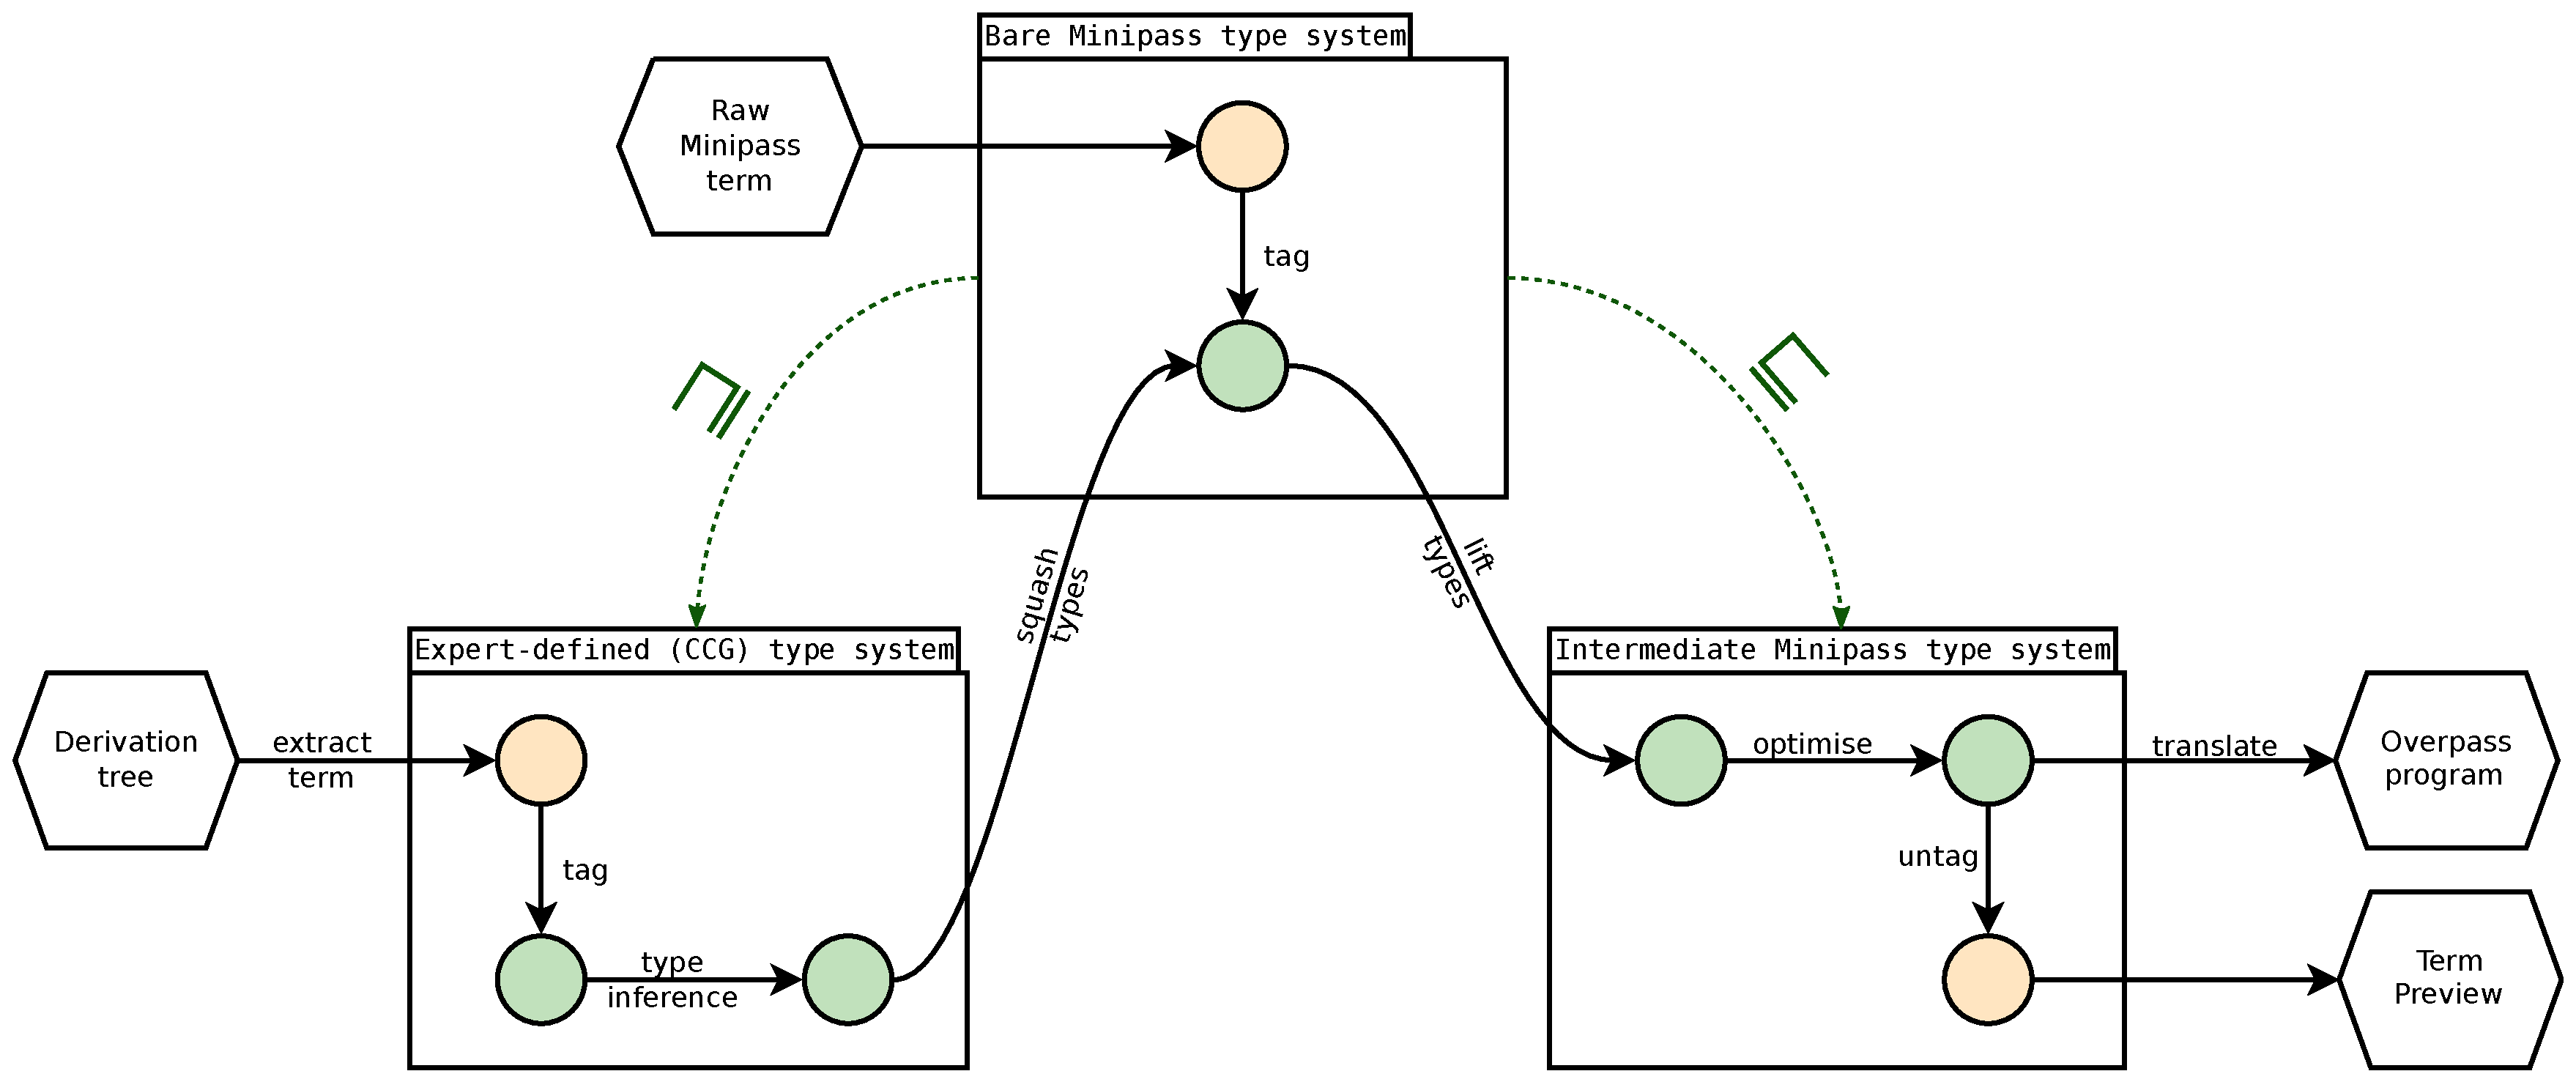
\includegraphics[width=\textwidth]{optimisation.eps}
    \caption{Illustration of the transformations a Minipass term undergoes}
    \label{fig:typesystems}
}

\subsubsection{Type inference}
\label{sec:typeinf}
Minipass allows for the usage of the special type \code{*} that acts as a
wildcard type. It violates the partial order of the type lattice since it is
equivalent to all types (i.e. $\forall \sigma \in T: (\text{\code{*}} \less \sigma)
\& (\sigma \less \text{\code{*}})$).

Thus, all significant\footnote{
    Since we only work with closed terms, the only case when a type can't be
    inferred is when a bound variable is unused (for example in terms like
    \code{(\textbackslash x, y => y) 42}, where the type of \code{x} cannot be inferred).
    This, however, is harmless, because the type is unneeded anyway.
} occurances of $\code{*}$ are removed by finding the fixed point of
$\mcf{propagate}$ from \cref{def:propagation}
with the following unifier:
\[
    \sigma \unify \tau =
    \begin{cases*}
        \tau ,& $\sigma = \text{\code{*}}$ \\
        \sigma ,& $\tau = \text{\code{*}}$ \\
        \sigma ,& $\sigma = \tau$ \\
        (\sigma' \unify \tau') \tot (\sigma'' \unify \tau'') ,&
            $\sigma = (\sigma' \tot \sigma''), \tau = (\tau' \tot \tau'')$ \\
        \lnot ! ,& $\mathsf{otherwise}$ \\
    \end{cases*}
\]

Whenever the algorithm encounters a case where the unifier is not defined,
a type error is produced.

Since this unifier can only change a subtype from \code{*} to something else,
and there are a finite number of subtypes within a term, this algorithm
always terminates.

\subsubsection{Minipass query optimisation}
\label{sec:optimisation}
\fixme{write this}

\subsubsection{Translating to Overpass}
\fixme{write this}
\end{document}
